\documentclass[oneside, 11pt]{article}

\usepackage[T1]{fontenc}
\usepackage[utf8]{inputenc}
\usepackage[dutch]{babel}

\usepackage{fouriernc}
\usepackage[detect-all, load-configurations=binary,
            separate-uncertainty=true, per-mode=symbol,
            retain-explicit-plus, range-phrase={ tot }]{siunitx}

\usepackage{setspace}
\setstretch{1.2}

\setlength{\parskip}{\smallskipamount}
\setlength{\parindent}{0pt}

\usepackage{geometry}
\geometry{marginparwidth=0.5cm, verbose, a4paper, tmargin=3cm, bmargin=3cm, lmargin=2cm, rmargin=2cm}

\usepackage{float}

\usepackage[fleqn]{amsmath}
\numberwithin{equation}{section}
\numberwithin{figure}{section}

\usepackage{graphicx}
\graphicspath{{Figures/}}
\usepackage{subfig}

\usepackage{tikz}
\usetikzlibrary{plotmarks}

\usepackage{fancyhdr}
\pagestyle{fancy}
\fancyhf{}
\rhead{\thepage}
\renewcommand{\footrulewidth}{0pt}
\renewcommand{\headrulewidth}{0pt}

\usepackage{relsize}
\usepackage{xspace}
\usepackage{url}

\newcommand{\figref}[1]{Figuur~\ref{#1}}

\newcommand{\hisparc}{\textsmaller{HiSPARC}\xspace}
\newcommand{\kascade}{\textsmaller{KASCADE}\xspace}
\newcommand{\sapphire}{\textsmaller{SAPPHiRE}\xspace}
\newcommand{\jsparc}{\textsmaller{jSparc}\xspace}
\newcommand{\hdf}{\textsmaller{HDF5}\xspace}
\newcommand{\aires}{\textsmaller{AIRES}\xspace}
\newcommand{\csv}{\textsmaller{CSV}\xspace}
\newcommand{\python}{\textsmaller{PYTHON}\xspace}
\newcommand{\corsika}{\textsmaller{CORSIKA}\xspace}
\newcommand{\labview}{\textsmaller{LabVIEW}\xspace}
\newcommand{\daq}{\textsmaller{DAQ}\xspace}
\newcommand{\adc}{\textsmaller{ADC}\xspace}
\newcommand{\adcs}{\textsmaller{ADC}s\xspace}
\newcommand{\Adcs}{A\textsmaller{DC}s\xspace}
\newcommand{\hi}{\textsc{h i}\xspace}
\newcommand{\hii}{\textsc{h ii}\xspace}
\newcommand{\mip}{\textsmaller{MIP}\xspace}
\newcommand{\hisparcii}{\textsmaller{HiSPARC II}\xspace}
\newcommand{\hisparciii}{\textsmaller{HiSPARC III}\xspace}
\newcommand{\pmt}{\textsmaller{PMT}\xspace}
\newcommand{\pmts}{\textsmaller{PMT}s\xspace}

\DeclareSIUnit{\electronvolt}{\ensuremath{\mathrm{e\!\!\:V}}}

\DeclareSIUnit{\unitsigma}{\ensuremath{\sigma}}
\DeclareSIUnit{\mip}{\textsmaller{MIP}}
\DeclareSIUnit{\adc}{\textsmaller{ADC}}

\DeclareSIUnit{\gauss}{G}
\DeclareSIUnit{\parsec}{pc}
\DeclareSIUnit{\year}{yr}



\begin{document}

\title{Dagelijkse controle van een station}
\author{C.G.N. van Veen} 
\date{}

\maketitle

\section{Stations}

\hisparc heeft verschillende meetstations op scholen in heel Nederland staan. 
Aangezien deze stations de hele dag meten en hun data verzenden naar de \hisparc database, moeten zij regelmatig gecontroleerd worden op correcte werking.
Informatie over de status van een station is te vinden op \url {http://data.hisparc.nl}.
Dit document geeft aan hoe te handelen als de status van een station niet optimaal is.

\section{Status van een station controleren}

Als contactpersoon van \hisparc bent u verantwoordelijk voor het onderhoud van het meetstation op uw school of instelling.
Om de prestaties van het station bij te houden, kunt u eens per dag kijken op de site: \url  {http://data.hisparc.nl}, waarvan in figuur \ref{fig:frontweb} een screenshot te zien is.
Op deze site staan alle stations, die in het netwerk van \hisparc zijn aangesloten, vermeldt. 
De cirkels voor de stations geven met een kleurcode aan wat de status van een station is. Als de kleur van de cirkel voor het betreffende station groen is, dan is de status van het station 'in orde'. 
Een gele cirkel geeft aan dat er een probleem is met het station. Een rode cirkel betekent dat er geen data van het station ontvangen wordt en dat het station dus niet werkt.

\begin{figure}
    \centering
    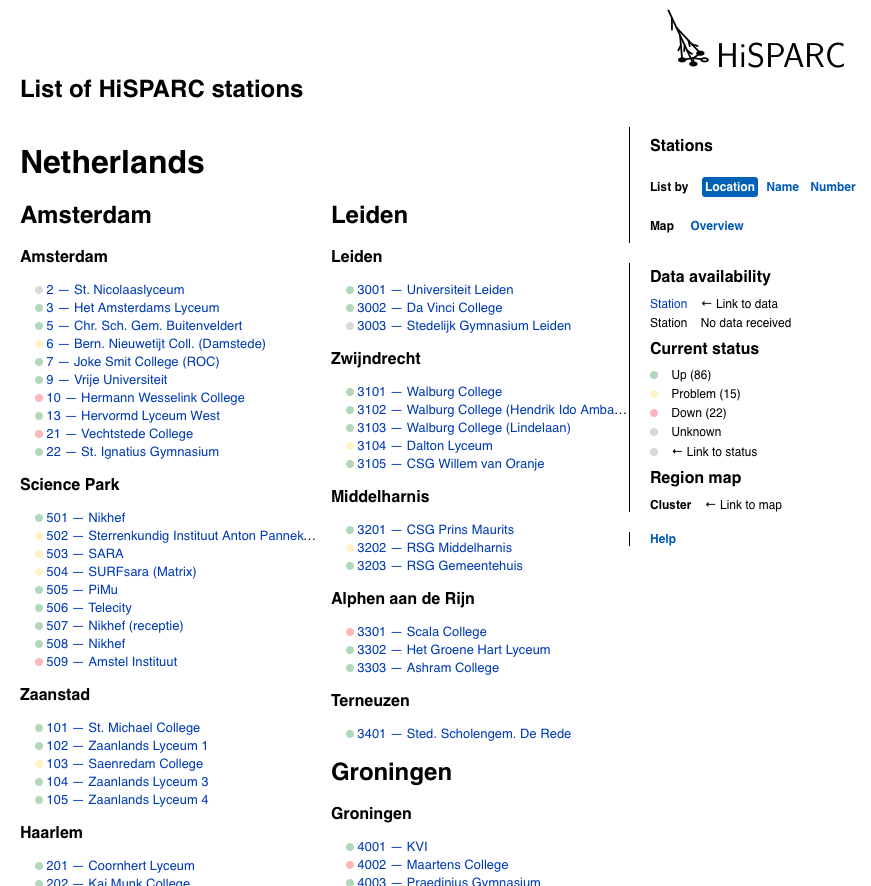
\includegraphics[scale=0.60]{websitefront}
    \caption{Vooraanzicht van de \hisparc website.}
   \label{fig:frontweb}
\end{figure}

\section{Probleem met een station}

In het geval van een gele cirkel, moet u klikken op de link van het desbetreffende station. Zie figuur \ref{fig:frontweb}.

 \begin{figure}
\centering
 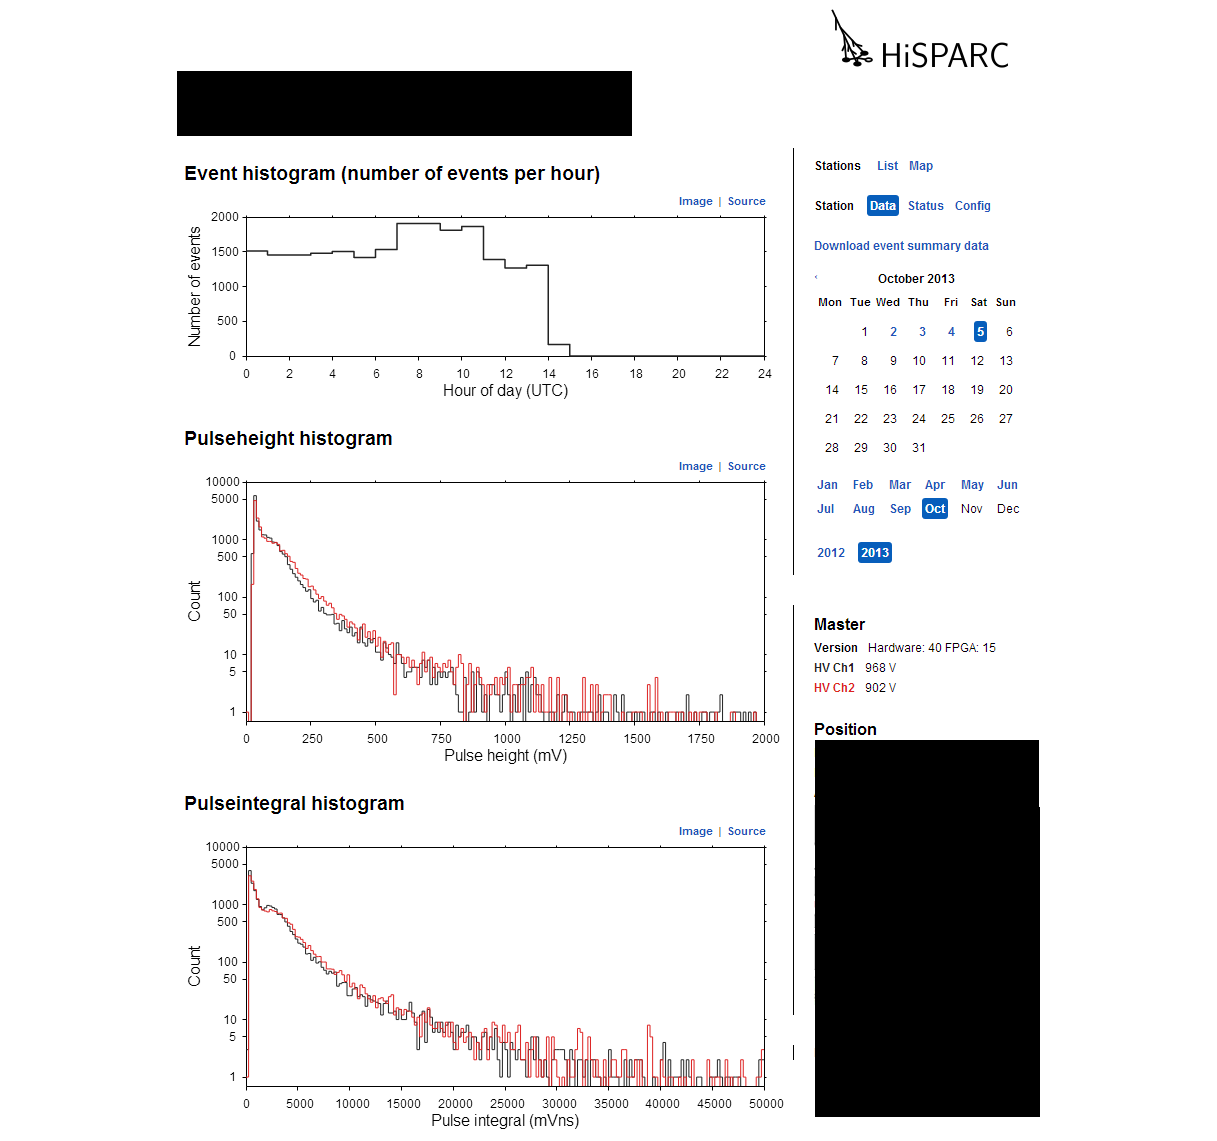
\includegraphics[scale=0.40]{websiteerror}
 \label{fig:websiteproble}
\caption{Screenshot van de status van een station. In het event histogram is duidelijk te zien dat het station niets meer meet
na 14.00 uur. Ook is er in het Pulseheight histogram geen duidelijke MIP piek te zien.}
\end{figure}




\begin{thebibliography}{9}
    \bibitem{Fokkema}
        D.B.R.A. Fokkema, \emph{The \hisparc Experiment, data acquisition and reconstruction of shower direction}, PhD. thesis 2012
\end{thebibliography}



\end{document}
